% DRAFT (05.11.2026), proposed replacement of main.tex, section "The k-bonacci
% Neighborhood" from \begin{definition} to the end of the "Positional DP" paragraph.
% Not yet in main.tex. Needs \usepackage{graphicx} and \newtheorem{lemma}{Lemma}.
% Figures: figures/fig_boards.tex, fig_tiling.tex, fig_share.tex (standalone).

\section{The $k$-bonacci Neighborhood}

\begin{definition}
Let $k\geq 2$. An \emph{elementary move} $s(i,j)$ with $1\leq j-i\leq k-1$
exchanges $\pi(i)$ and $\pi(j)$ and leaves $\pi(i+1),\dots,\pi(j-1)$ in
place. A \emph{compound move} is a set of elementary moves whose
intervals $[i,j]$ are pairwise disjoint. $\N_k(\pi)$ is the set of
permutations reachable by one compound move.
\end{definition}

For $k=2$ only adjacent jobs are exchanged, which gives the Fibonacci
neighborhood. For $k=3$ a swap may also skip one job (tribonacci), and for
$k=n$ any two jobs may be exchanged, which gives Dynasearch.

\paragraph{Moves as rook placements.} A compound move is a permutation
$\sigma$ of the positions, so it can be drawn as its permutation matrix:
$n$ non-attacking rooks on an $n\times n$ board, one in each row and
column, with a rook in cell $(t,\sigma(t))$. Every elementary move is a transposition and the
transpositions of one compound move have disjoint supports, so $\sigma$ is
an involution and its board is symmetric about the main diagonal. For
$L\geq 2$ let $S_L$ be the $L\times L$ identity matrix with the two corner
ones moved to $(1,L)$ and $(L,1)$, and let $S_1=[1]$.

\begin{lemma}\label{lem:blocks}
$\sigma\in\N_k$ if and only if its permutation matrix is block diagonal,
$P_\sigma=\mathrm{diag}(S_{L_1},\dots,S_{L_r})$, with
$L_1+\dots+L_r=n$ and every $L_q\leq k$. The block sizes are determined
by $\sigma$.
\end{lemma}
\begin{proof}
A swap $s(i,j)$ acts only on positions $i..j$, so it is the block
$S_{j-i+1}$ placed on the diagonal at rows $i..j$. Disjoint intervals
give disjoint diagonal blocks, and the untouched positions are blocks
$S_1$. Conversely, each block $S_L$ with $2\leq L\leq k$ is one swap of
distance $L-1\leq k-1$. A block $S_L$ with $L\geq 2$ cannot be split,
because its corner rooks link row $1$ with column $L$, so the
decomposition is unique.
\end{proof}

Figure~\ref{fig:boards} shows the four cases side by side. In the
Fibonacci board the rooks stay on the diagonal or in $2\times 2$ blocks
next to it. Raising $k$ widens the band $|t-\sigma(t)|\leq k-1$ that the
rooks may occupy, and for $k=n$ the band covers the whole board. The
block structure is the second constraint, and the band alone does not
imply it: the $3$-cycle $\sigma=(2,3,1)$ stays within the band of $k=3$
but is not an involution. The Motzkin neighborhood~\cite{motzkin_own}
relaxes the block structure in a different way. It allows a swap inside
the interval of another swap (dashed block in Fig.~\ref{fig:boards}), as
long as no two intervals cross.

\begin{figure}[t]
\centering
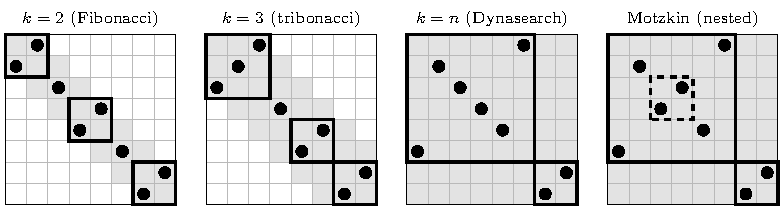
\includegraphics[width=\linewidth]{figures/fig_boards.pdf}
\caption{One compound move of each neighborhood for $n=8$, drawn as rooks
on the board. Shaded cells form the band $|t-\sigma(t)|\leq k-1$ and
thick squares mark the diagonal blocks of Lemma~\ref{lem:blocks}.}
\label{fig:boards}
\end{figure}

\paragraph{Counting.} Lemma~\ref{lem:blocks} turns a compound move into
a sequence of block sizes, that is, a tiling of positions $1..n$ by tiles
of length $1$ to $k$ (Fig.~\ref{fig:tiling}a). Fixing the length $L$ of
the first tile leaves an arbitrary move on the remaining $n-L$ positions
(Fig.~\ref{fig:tiling}b), which yields the $k$-bonacci recurrence.

\begin{proposition}\label{prop:count}
$|\N_k(\pi)|=a_n$, where $a_0=1$ and $a_p=\sum_{L=1}^{\min(k,p)}a_{p-L}$.
The generating function is $\sum_{p\geq 0}a_p x^p=1/(1-x-x^2-\dots-x^k)$.
Hence $|\N_2|=F_{n+1}$, $|\N_n|=2^{n-1}$, and
$|\N_k|=\Theta(\lambda_k^n)$, where $\lambda_k$ is the largest real root
of $x^k=x^{k-1}+\dots+x+1$. Moreover $2-\lambda_k=\lambda_k^{-k}$, so
$\lambda_k=2-\Theta(2^{-k})$.
\end{proposition}
\begin{proof}[Sketch]
The recurrence and the generating function follow from the first-tile
decomposition, and distinct tilings give distinct permutations by
Lemma~\ref{lem:blocks}. Multiplying
$x^k=(x^k-1)/(x-1)$ by $x-1$ gives $x^{k+1}-2x^k+1=0$, that is,
$2-x=x^{-k}$.
\end{proof}

\begin{figure}[t]
\centering
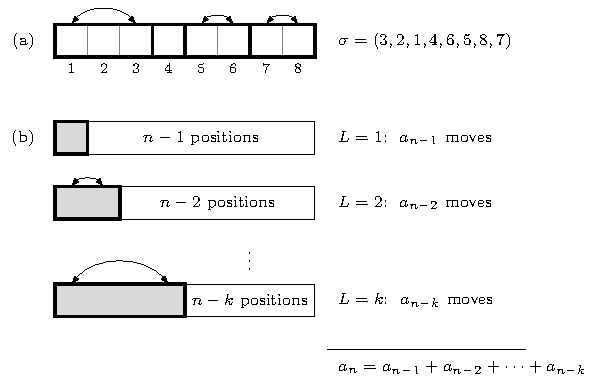
\includegraphics[width=0.8\linewidth]{figures/fig_tiling.pdf}
\caption{(a) The $k=3$ move of Fig.~\ref{fig:boards} as a tiling;
arrows join the swapped jobs. (b) The first tile has length
$L\in\{1,\dots,k\}$ and leaves a move on $n-L$ positions.}
\label{fig:tiling}
\end{figure}

\paragraph{The hierarchy.} A move of $\N_k$ is also a move of
$\N_{k+1}$, and the inclusion is strict whenever $k<n$, because a single
swap of distance $k$ lies in $\N_{k+1}$ only. Together with the
neighborhoods of the earlier studies this gives the chain
\begin{equation}\label{eq:chain}
\N_{\mathrm{adj}}\subset\N_2=\N_{\mathrm{fib}}\subset\N_3\subset\dots
\subset\N_n=\N_{\mathrm{dyn}}\subset\N_{\mathrm{mot}}\subset\mathcal I_n,
\end{equation}
where $\mathcal I_n$ is the set of all involutions. On the board, the
first part of the chain widens the band, the step to Motzkin allows nested
blocks, and the last step allows crossing swaps. For $n=10$ the sizes are
$89$, $274$, $401$, $492$ and $512$ for $k=2,3,4,6,n$, then $2188$ for
Motzkin and $9496$ for all involutions.
\todo{check whether \cite{bozejko2026sr} or the IFAC 2025 paper already
state this chain; Fibonacci and Motzkin are joint work with the
supervisor}

\paragraph{How much of Dynasearch does $\N_k$ cover?} Every Dynasearch
move is a composition of $n$, and a uniformly random composition places
an independent cut between neighboring positions with probability $1/2$.
A block of length $L$ is then a run of $L-1$ positions without a cut, so
the share $|\N_k|/2^{n-1}$ is the probability that $n-1$ fair coin flips
contain no run of $k$ consecutive gaps without a cut. By the classical
longest-run law this probability jumps from near $0$ to near $1$ around
$k=\log_2 n$ (Fig.~\ref{fig:share}). For $k=\lfloor\log_2 n\rfloor+2$ the
share is $0.79$--$0.89$ for $n=20$--$500$, whereas for any constant $k$
it vanishes exponentially. A moderate $k$ therefore keeps most Dynasearch
moves and drops only the rare moves with very long swaps.

\begin{figure}[t]
\centering
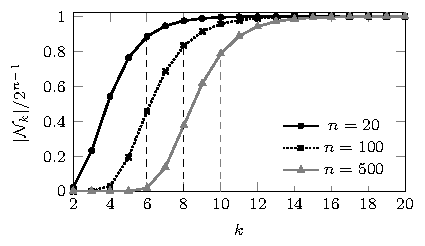
\includegraphics[width=0.6\linewidth]{figures/fig_share.pdf}
\caption{Share of Dynasearch moves contained in $\N_k$. Dashed lines mark
$k=\lfloor\log_2 n\rfloor+2$.}
\label{fig:share}
\end{figure}

\paragraph{Evaluation.} For every candidate $(i,j)$ we compute
$\delta_{ij}=C_{\max}(\pi\circ s(i,j))-C_{\max}(\pi)$ with heads and
tails. The candidates are the cells of the band above the diagonal,
$(k-1)n-k(k-1)/2<n(k-1)$ of them, against $n(n-1)/2$ for Dynasearch. A
candidate of distance $d$ costs $O(md)$, so all deltas cost $O(mnk^2)$
instead of $O(mn^3)$. Candidates are filtered with the block-boundary
test used for the Fibonacci, Dynasearch and Motzkin neighborhoods in the
earlier studies~\cite{windowed_own}: a swap $(i,j)$ is kept only if a
boundary position lies in $[i,j]$. \todo{wording of the filter: decision
on the exact critical-path variant (see plan, \S14)}

\paragraph{Positional DP.} Let $B[p]$ be the minimum total delta of a
compound move restricted to positions $1..p$. By Lemma~\ref{lem:blocks}
the last block ends at $p$ and has length $1$ or $d+1\leq k$, so
\begin{equation}
B[p]=\min\Bigl(B[p-1],\ \min_{1\le d\le k-1} B[p-d-1]+\delta_{p-d,p}\Bigr),
\end{equation}
with $B[0]=0$, which takes $O(nk)$ time and memory. When no move improves
the predicted makespan, the best single swap is applied, as in the
Dynasearch and Motzkin neighborhoods.
